\chapter{Arquitetura RAMCloud}
\label{ch:3}


\begin{figure}[H]
\begin{minted}[frame=single,linenos,mathescape,fontsize=\scriptsize,label=exemplo.list]{py3}
# Lista de professores (linhas de comentarios comecam com '#')
4575931307749163,Carlos Hitoshi Morimoto, 1999-HOJE, Professor
0131770792108992,Joao Eduardo Ferreira, 1999-2006 & 2006-HOJE, Professor
0362417828475021,Junior Barrera, 1992-2008, Professor
0926213060635986,Marcel Parolin Jackowski, 2006-HOJE, Professor
0644408634493034,Nina Sumiko Tomita Hirata,,Professor # membro sem periodo
1647118503085126,Roberto Hirata Junior,, Professor # membro sem periodo
2240951178648368,Roberto Marcondes Cesar Junior, 1998-HOJE, Professor
9283304583756076,Ronaldo Fumio Hashimoto,, Professor # membro sem periodo

# lista de colaboradores
4727357182510680,Jesus P. Mena-Chalco, 1995-1999 & 2005-HOJE, Colaborador

# lista de alunos
2837012019824386,Andrea Britto Mattos,, Aluno# membro sem periodo
\end{minted}
\caption{Arquivo de configuração do ScriptLattes que contém a lista de pesquisadores}
\label{lst:slattes}
\end{figure}


\begin{figure}[H]
    \centering 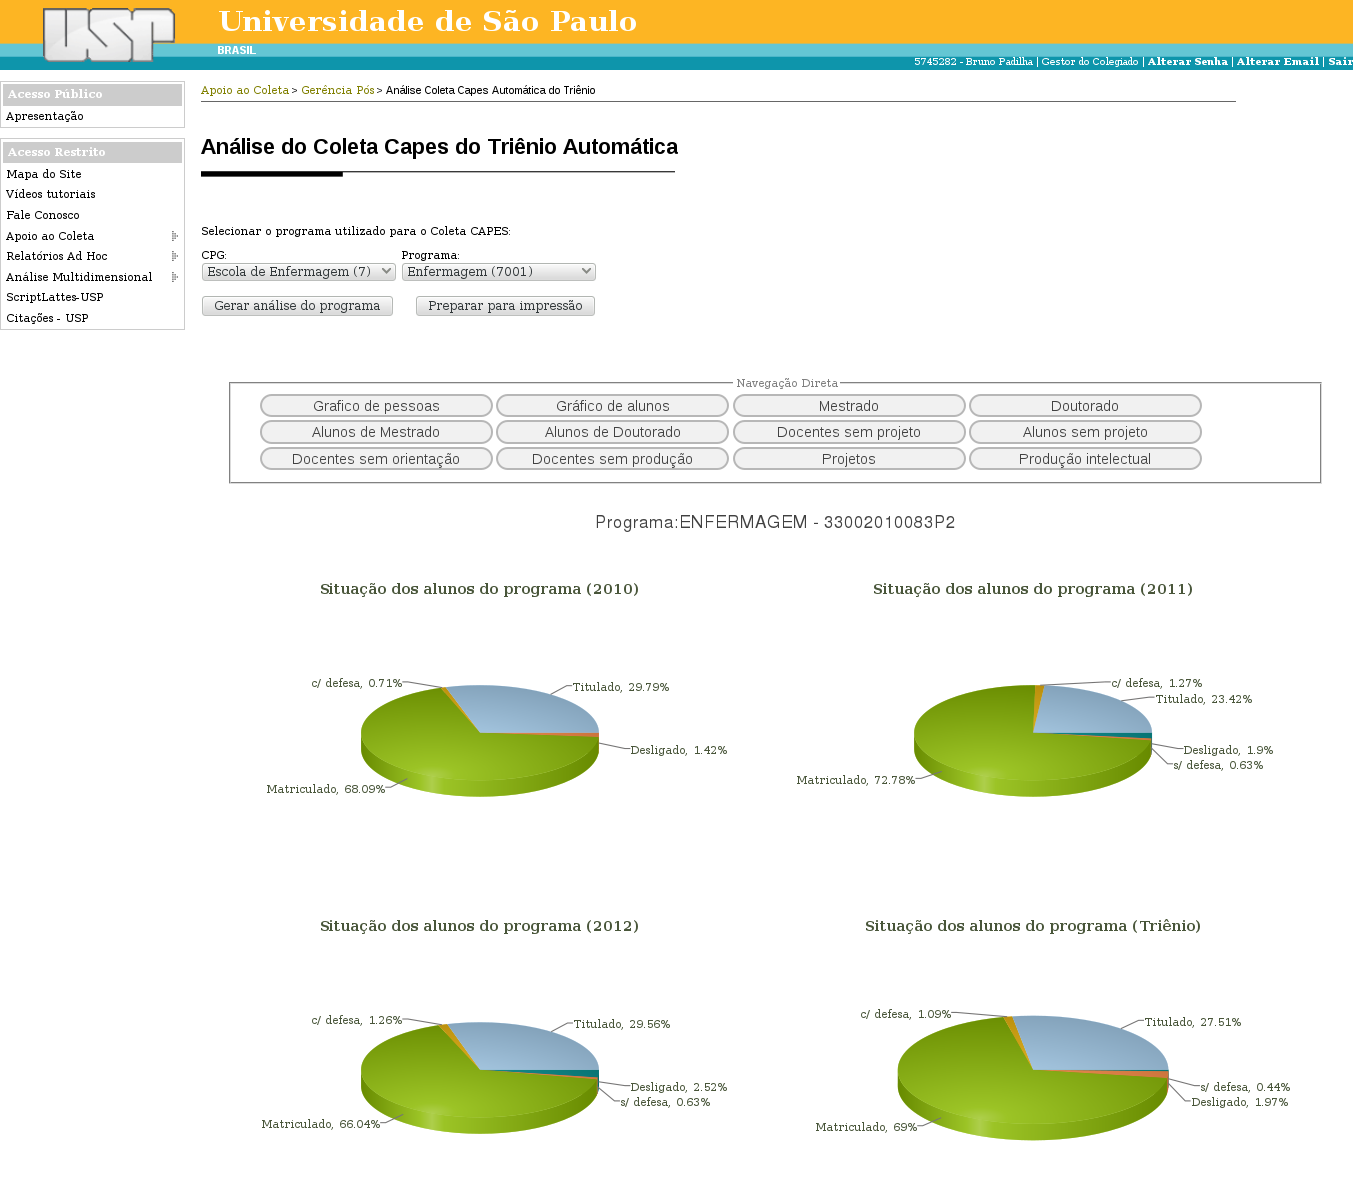
\includegraphics[width=0.5\textwidth]{figuras/trienio.png}
    \caption{Imagem parcial do relatório de análise do triênio}
    \label{fig:trim}
\end{figure} 

